% Chapter 6 text
\chapter{Rapid microbial oxidation of rock-derived organic carbon in mountain soils}
\label{Ch6}
\raggedbottom

{\let\thefootnote\relax\footnotetext{This chapter is currently in preparation for submission as: Hemingway J.D., Hilton, R.G., Hovius, N., Eglinton, T.I., and Galy V.V. {Rapid microbial oxidation of rock-derived organic carbon in mountain soils.}}}

\clearpage

\section{Abstract}

Over geologic timescales, oxidation of organic carbon contained in sedimentary rocks (OC\sub{petro}) is a major source of \ce{CO2} to the atmosphere. However, the governing mechanisms, rates, and sensitivity of OC\sub{petro} oxidation to changing environmental conditions such as erosion remain poorly constrained. Microbially mediated respiration of high-OC black shale and subsequent incorporation into biomass has been observed in laboratory-based incubation studies, suggesting that biotic processes might be an important factor. Here, we use geochemical characterizations of soils and fluvial suspended sediments from the highly erosive Central Range (Taiwan) to demonstrate the importance of microbial OC\sub{petro} oxidation. Using a combination of bulk OC, biomarkers, and the novel Ramped PyrOx (RPO) serial oxidation radiocarbon technique, we show that $73^{+2}_{-3}$ \% of OC initially present in bedrocks is oxidized to \ce{CO2}, and that the remainder is chemically altered during microbial assimilation in soils. This corresponds to a \ce{CO2} emission flux of \SIrange{5.6}{17.1}{t.C.km^{-2}.yr^{-1}} within the study region, consistent with independent estimates. Our results indicate that microbially mediated OC\sub{petro} oxidation is not kinetically limited despite high erosion rates and short residence times within the weathering front, suggesting that erosion exhibits a first-order control on OC\sub{petro} oxidation flux within mountain soils.

\section{Main text}

Oxidative weathering of organic carbon contained in sedimentary and meta-sedimentary rocks ("petrogenic" OC; OC\sub{petro}) is a major atmospheric \ce{CO2} source and \ce{O2} sink over geologic timescales \citep[\SI{\geq e6}{yr};][]{Berner:1989vr,Wildman:2004wf,Hayes:2006ca,Petsch:2014ct}. Because the reservoir of OC\sub{petro} available for oxidation (\textit{i.e.} contained in the upper $1$ m of continental surfaces) is roughly double that of atmospheric \ce{CO2} \citep{Copard:2007bf}, small relative perturbations in weathering rates may have a significant impact on the balance between \ce{CO2} production and drawdown. Alongside geological \ce{CO2} emissions from volcanism \citep{Marty:1998vo}, metamorphic outgassing \citep{Becker:2008bd}, and pyrite oxidation-driven weathering of carbonate minerals \citep{Torres:2014cx}, this flux must be compensated by burial in marine sediments of biospheric OC \citep[OC\sub{bio};][]{FranceLanord:1997ua,Galy:2007ev,Hilton:2008fo}, pyrite \citep{Berner:1989vr,Hayes:2006ca}, and/or carbonate minerals derived from chemical weathering of silicate rocks \citep{Berner:1989vr} in order to avoid imbalances that could drastically change atmospheric \ce{CO2} content \citep{Berner:1997df}. Despite their importance in balancing the global C cycle, \ce{CO2} emissions due to OC\sub{petro} oxidation are under-constrained, with model-based estimates ranging from \SIrange{38e6}{100e6}{t.C.yr^{-1}} \citep{Petsch:2014ct}. Furthermore, the relative importance of potential factors such as kinetic limitation \citep{Chang:1999vo,Petsch:2001eq}, physical erosion rate \citep{Hilton:2014dh}, and OC\sub{petro} chemical composition \citep{Galy:2008ff} remains unknown, hindering our ability to predict the response of OC\sub{petro} oxidation to changing environmental conditions.

Respiration and incorporation into microbial biomass has been proposed as one mechanism to explain the observed loss of OC\sub{petro} across a shale weathering front \citep{Petsch:2001eq,Petsch:2005gd,Schillawski:2008ko,Petsch:2014ct} and in exhumed glacial foreland soils \citep{Bardgett:2007eb}. However, all current constraints on this mechanism are derived from high-\%OC\sub{petro} black shale incubations in the laboratory \citep{Petsch:2001eq,Schillawski:2008ko}. Thus, the role of microbially mediated OC\sub{petro} weathering has yet to be evaluated in the field, especially in the low-\%OC\sub{petro} (\textit{i.e.} \SI{\leq 1}{\%}) environments that typify most sedimentary rock formations \citep{Copard:2007bf}. Furthermore, it has been suggested that OC\sub{petro} weathering rate constants may be $~10\times$ faster than those for silicate weathering \citep{Chang:1999vo}, potentially leading to an OC\sub{petro} oxidation flux that is supply limited and can thus keep pace with high erosion rates in mountainous environments \citep{Hilton:2014dh}. We provide new constraints on OC\sub{petro} weathering using soils from a highly erosive mountain belt: Central Range, Taiwan (Figure \ref{Ch6Fig:S1}). There, thin soils \citep[\SI{\leq 0.8}{m};][]{Tsai:2001vp} overlay meta-sedimentary rocks containing \SIrange{\approx 0.2}{0.4}{\%OC_{petro}} \citep[Supplementary Discussion \ref{Ch6SD1};][]{Hilton:2010cg}. High rates of river incision and bedrock landsliding due to tectonic uplift and frequent typhoon landfall lead to soil residence times on the order of centuries, thus providing an ideal environment to test the kinetic limits of microbial OC\sub{petro} respiration rates.

To do so, we analyzed a set of soils, including organic (A+E) and saprolite (C) horizons, bedrocks, and fluvial total suspended sediments (TSS) from the LiWu and WuLu catchments on the eastern flank of the Central Range (Figure \ref{Ch6Fig:S1}). Well-characterized OC\sub{petro} and OC\sub{bio} yields by these rivers \citep{Hilton:2008fo,Hilton:2010cg,Hilton:2011jw,Hilton:2012dt} as well as previous estimates of catchment-wide OC\sub{petro} oxidation rates using the trace element rhenium \citep{Hilton:2014dh}, provide a framework in which to interpret our results. Soil samples span a range of lithologies (Tananao schist, Lushan and Pilushan sedimentary formations), depths (\SIrange{0.0}{0.9}{m}), slope angles (\ang{1} to \ang{50}), and elevations (\SIrange{122}{3192}{m}) that are representative of the mountain belt \citep{Hilton:2013kq}. Additionally, we analyze TSS samples collected from the LiWu River during three successive typhoon events. The intense rainfall during these events erodes soils and bedrocks from throughout the catchment, providing an integrated view of weathering and erosion products \citep{Hilton:2010cg}. To quantify OC\sub{petro} loss, we measured bulk soil and TSS particulate OC (POC) carbon content, stable carbon isotope composition (reported as \ce{\delta^{13}C}), and \ce{^{14}C} activity \citep[reported as fraction modern (Fm) following][Table \ref{Ch6Tab:S1}--\ref{Ch6Tab:S2}]{Stuiver:1977uh}. In addition, we extracted and measured the concentrations, \ce{\delta^{13}C} values, and Fm values of long-chain \textit{n}-alkanoic acids ($\Sigma$LC\sub{24+}) as a tracer of OC\sub{bio} composition \citep{Eglinton:1967uz}, as well as the concentrations and \ce{\delta^{13}C} values of the microbially produced \textit{i}-C\sub{15} and \textit{a}-C\sub{15} alkanoic acids \citep{Bardgett:2007eb} from all soils and a subset of TSS samples (Supplementary Methods \ref{Ch6M}; Table \ref{Ch6Tab:S3}--\ref{Ch6Tab:S5}).

To provide new insight into the fate of OC\sub{petro} during weathering, we relate the chemical and isotope composition of OC using the Ramped PyrOx (RPO) serial oxidation technique \citep{Rosenheim:2008ed,Rosenheim:2012kh}. This method separates OC based on the decomposition temperature when heated at a constant ramp rate (\textit{i.e.} OC thermal lability) and provides \ce{\delta^{13}C} and Fm values for material that has decomposed over user-defined temperature "fractions" (Supplementary Methods \ref{Ch6M}). We transpose the thermal profiles into activation energy ($E$) space, an intrinsic property of chemical bonding environment and thus a proxy for OC chemical structure, using an inverse distributed activation energy kinetic model (Table \ref{Ch6Tab:S6}; Supplementary Discussion \ref{Ch6SD2}; Chapter \ref{Ch3}). The mean $E$ value for each RPO fraction can be interpreted alongside its corresponding \ce{\delta^{13}C} and Fm values in order to track multiple sources of OC within a single sample \citep{Rosenheim:2008ed,Rosenheim:2012kh}.

% Figure 1
\begin{figure}[t]
	\makebox[\textwidth][c]{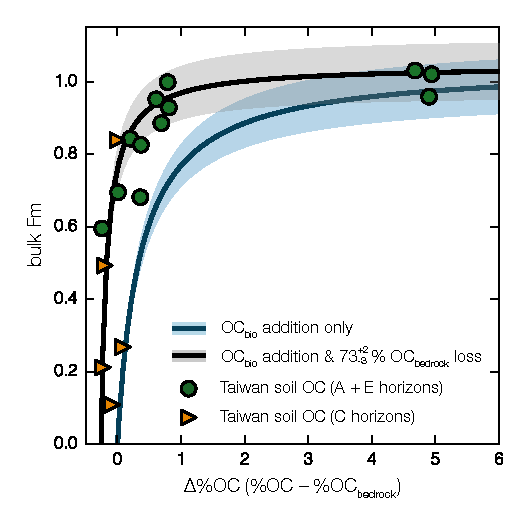
\includegraphics[]{Thesis_Figures/Ch6Fig1}}
	\caption[Bulk $\Delta$\%OC vs. Fm mixing plot]{Bulk end-member mixing model indicating the loss of OC\sub{petro} in Taiwanese C-horizon (orange traingles) and A+E-horizon (green circles) soils. Blue line represents the trend expected if no OC\sub{petro} were oxidized (\textit{i.e.} OC\sub{bio} addition only) using an Fm\sub{bio} value of \num{1.045 \pm 0.079} derived from \textit{n}-alkanoic acid Fm values (Table \ref{Ch6Tab:S5}). Black line represents the trend using the same Fm\sub{bio} value for the best-fit fraction of OC\sub{petro} oxidized ($73^{+2}_{-3}$ \%; RMSE $= 0.22$). Shading region for both trends is $\pm 1\sigma$ propagated from Fm\sub{bio} uncertainty. See Supplemental Discussion \ref{Ch6SD4} for mixing model derivation.}
	\label{Ch6Fig:1} 
\end{figure}

OC\sub{petro} oxidation is evident throughout the soil dataset due to the fact that some samples contain lower \%OC than that of the unweathered bedrock material (\%OC\sub{br}) immediately underlying them (\textit{i.e.} $\Delta$\%OC = \%OC -- \%OC\sub{br} $< 0$; Figure \ref{Ch6Fig:1}). Using a mean \%OC\sub{br} value for the sample set of \SI{0.36 \pm 0.16}{\%} and modelling bulk soil Fm as an admixture of OC\sub{bio} (Fm\sub{bio} = \num{1.045 \pm 0.079}; Table \ref{Ch6Tab:S5}; Supplementary Discussion \ref{Ch6SD3}) with residual OC\sub{petro} (Fm\sub{petro} $\equiv 0.0$), these data are consistent with an average of $73^{+2}_{-3}$ \% OC\sub{br} loss during soil formation (Figure \ref{Ch6Fig:1}). Comparison between two samples collected at different depths from the same saprolite sequence provides direct evidence for significant oxidation of OC\sub{petro} and replacement by OC\sub{bio} within the C-horizon of soils \citep{Hilton:2013kq}. These samples, collected from \SI{0.2}{m} and \SI{0.5}{m} depth, contain nearly identical \%OC values (\SI{0.20}{\%} and \SI{0.28}{\%}) but drastically different radiocarbon content (Fm = $0.108$ and $0.839$; Table \ref{Ch6Tab:S2}). Therefore, despite denudation rates of \SIrange{3}{6}{mm.yr^{-1}} \citep{Dadson:2003kl} and shallow soils \citep[\SI{\leq 0.8}{m};][]{Tsai:2001vp}, OC\sub{petro} appears to be mostly weathered before soil A+E horizons have fully developed. This suggests that oxidation is not kinetically limited in these settings \citep[\textit{c.f.}][]{Chang:1999vo,Petsch:2001eq}, consistent with the idea that biology can drive rapid weathering in young soils with abundant nutrients and that the weathering front progresses with physical denudation \citep{Brantley:2011ku}.

Using this result and an area-weighted average \%OC\sub{br} value for the WuLu and LiWu catchments of \SI{0.24 \pm 0.06}{\%} \citep{Hilton:2010cg}, we calculate the annual \ce{CO2} flux resulting from OC\sub{petro} oxidation in soils using a Monte Carlo approach with three independent residence time estimates (Supplementary Discussion \ref{Ch6SD4}). These measurements of OC\sub{petro} loss from soils suggest a median atmospheric \ce{CO2} flux of \SIrange{5.6}{17.1}{t.C.km^{-2}.yr^{-1}} (Figure \ref{Ch6Fig:S2}A), consistent with previous estimates for Taiwan: $(i)$ \SI{\leq 12}{t.C.km^{-2}.yr^{-1}} calculated by comparing riverine OC\sub{petro} yield and TSS yield \citep[Figure \ref{Ch6Fig:S2}B;][]{Hilton:2011jw}, and $(ii)$ \SIrange{7}{13}{t.C.km^{-2}.yr^{-1}} calculated using dissolved rhenium yield as a proxy for OC\sub{petro} oxidation \citep[Figure \ref{Ch6Fig:S2}B;][]{Hilton:2014dh}. While similar within uncertainty, our estimates are slightly lower than catchment-specific rhenium-based values, and may suggest additional OC\sub{petro} oxidation in locations not captured by our soil samples such as landslide colluvium \citep{Emberson:2016fp} and/or during fluvial transit \citep{Galy:2008ff}. This flux is on the same order of magnitude as \ce{CO2} drawdown due to OC\sub{bio} export from rivers combined with subsequent burial in marine sediments [Taiwan average: \SI{21 \pm 10}{t.C.km^{-2}.yr^{-1}}; Figure \ref{Ch6Fig:S2}C; \citealp{Hilton:2012dt}] as well as that due to weathering of silicate minerals \citep[LiWu River: \SI{7.04}{t.C.km^{-2}.yr^{-1}}; Figure \ref{Ch6Fig:S2}D;][]{Calmels:2011gv}. OC\sub{petro} oxidation in thin mountain soils is therefore a quantitatively important process in setting the net role of these systems within the global carbon cycle.

% Figure 2
\begin{figure}[p]
	\makebox[\textwidth][c]{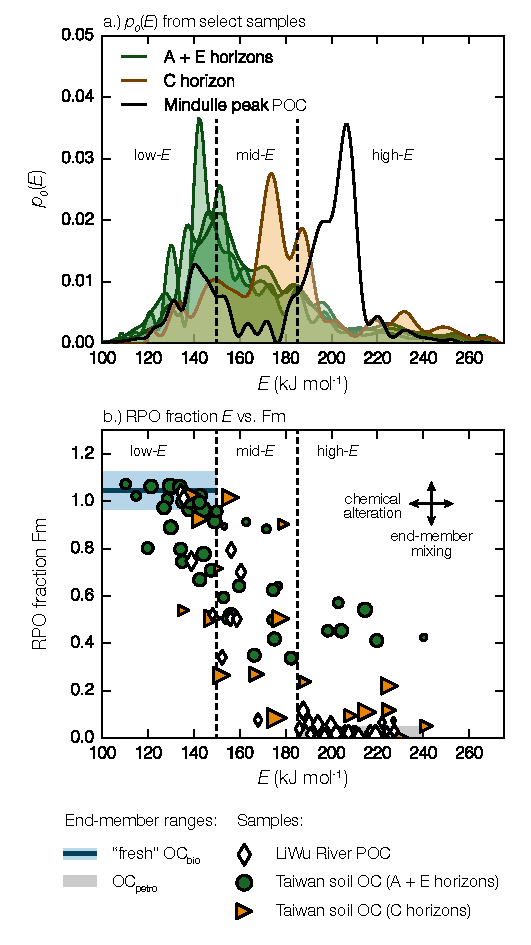
\includegraphics[]{Thesis_Figures/Ch6Fig2}}
	\caption[RPO $p_{0}(E)$ distributions and $E$ vs. Fm plots]{\textit{(A)} RPO-derived $E$ distributions [$p_{0}(E)$] for LiWu River POC during the peak of Typhoon Mindulle \citep[white;][]{Hilton:2008fo}, a representative C-horizon soil (orange), and an A+E horizon soil profile (green) calculated using the inverse distributed activation energy model of Chapter \ref{Ch3}. \textit{(B)} Relationship between Fm and mean $E$ for each RPO fraction from all measured LiWu River POC (white diamond), C-horizon soil (orange diamond), and A+E-horizon soil (green circle) samples (Table \ref{Ch6Tab:S6}). End-member regions are plotted as a blue envelope for fresh OC\sub{bio} (Fm\sub{bio} = \num{1.045 \pm 0.079}; $E$ \SI{< 150}{kJ.mol^{-1}}; Table \ref{Ch6Tab:S5}) and a gray box for OC\sub{petro} ($E$ \SI{\geq 185}{kJ.mol^{-1}}). Marker size represents the relative amount of OC contained in each RPO fraction. Black arrows represent the trends expected for end-member mixing (vertical) and chemical alteration due to microbial OC\sub{petro} assimilation (horizontal, left) or OC\sub{bio} condensation (horizontal, right) in Fm vs. $E$ space. For both panels, dotted lines separate $p_{0}(E)$ into low-$E$ (\SI{<150}{kJ.mol^{-1}}), mid-$E$ ($150 \leq E < 185$ \si{kJ.mol^{-1}}), and high-$E$ (\SI{\geq 185}{kJ.mol^{-1}}) regions.}
	\label{Ch6Fig:2} 
\end{figure}

RPO results provide strong evidence that OC\sub{petro} remaining in soils has been chemically altered during weathering, as can be seen by comparing the probability density function (pdf) of $E$ [$p_{0}(E)$] for fluvial POC versus C-horizon and A+E-horizon soil OC (Figure \ref{Ch6Fig:2}A). Because $E$ is a proxy for OC chemical bonding environment, $p_{0}(E)$ represents the distribution of chemical bonds within a sample (Supplementary Discussion \ref{Ch6SD2}; Chapter \ref{Ch3}). To constrain $p_{0}(E)$ for unweathered OC\sub{petro}, we calculate the average of all LiWu TSS samples (including isolated \SI{\geq 2}{mm} clasts; $n = 27$; Figure \ref{Ch6Fig:S3}A), as bulk Fm values indicate that POC in these samples is mostly petrogenic in origin \citep[Table \ref{Ch6Tab:S1};][]{Hilton:2008fo,Hilton:2010cg,Hilton:2011jw}. Results indicate that unweathered OC\sub{petro} is exclusively associated with $E$ values above \SI{185}{kJ.mol^{-1}} (termed "high-$E$"), consistent with the fact that it is predominantly composed of highly condensed and reduced aromatic material \citep{Galy:2008ff}. In contrast, vascular-plant-derived (\textit{i.e.} "fresh") OC\sub{bio}, which dominates the surface A+E horizon soils (as demonstrated by their high \%OC, bulk Fm, and $\Sigma$LC\sub{24+} \textit{n}-alkanoic acid concentrations, Table \ref{Ch6Tab:S2}--\ref{Ch6Tab:S3}), is described by a $p_{0}(E)$ distribution centered at much lower $E$ values. We constrain fresh OC\sub{bio} $p_{0}(E)$ using two organic-rich surface soils that exhibit nearly modern Fm values \citep[\%OC \SI{> 5}{\%}, Fm $> 0.96$; Table \ref{Ch6Tab:S2};][]{Hilton:2013kq}. For both samples \SI{> 90}{\%} of OC is associated with $E$ \SI{< 150}{kJ.mol^{-1}} (termed "low-$E$"), indicating OC\sub{petro} and OC\sub{bio} can be clearly separated in terms of their $E$ values (Figure \ref{Ch6Fig:S3}). 

C-horizon saprolites and deeper A+E-horizon soils contain a significant amount of OC associated with $E$ values between \SIrange{150}{185}{kJ.mol^{-1}} ("mid-$E$"; Figure \ref{Ch6Fig:2}A, \ref{Ch6Fig:S3}B), higher than that observed in fresh OC\sub{bio} yet lower than OC\sub{petro}. Importantly, a binary mixing of fresh OC\sub{bio} and OC\sub{petro} cannot explain this result, as this would instead lead to a bimodal $p_{0}(E)$ distribution (\textit{e.g.} Mindulle peak POC, Figure \ref{Ch6Fig:2}A). Rather, this phenomenon can derive either from an increase in aromaticity of fresh OC\sub{bio} (\textit{i.e.} increased thermal recalcitrance, with a small contribution due to charring within the RPO instrument; Supplementary Discussion \ref{Ch6SD2}) and/or an increase in the oxidation state of remaining OC\sub{petro} after weathering \citep[\textit{i.e.} decreased thermal recalcitrance; Chapter \ref{Ch3}][]{Williams:2014bq}. These processes can be distinguished using the \ce{^{14}C} activity of each RPO faction, as low-$E$ Fm values for both soils and POC cluster near the fresh OC\sub{bio} end-member (as estimated by $\Sigma$LC\sub{24+} \textit{n}-alkanoic acid Fm; Supplementary Methods \ref{Ch6M}; Table \ref{Ch6Tab:S6}), while high-$E$ RPO fractions for POC and C-horizon soils cluster near Fm $= 0.0$ (\textit{i.e.} OC\sub{petro}; Figure \ref{Ch6Fig:2}B). In contrast, mid-$E$ RPO fractions span the entire range of Fm values from $0.076$ to $1.016$ (average = \num{0.566 \pm 0.254}; Table \ref{Ch6Tab:S6}). This component can become quantitatively important in soils, with the relative amount of OC contained in the mid-$E$ region ($f_{\text{mid}}$) reaching \SI{51}{\%} in saprolite sequences (Supplementary Discussion \ref{Ch6SD2}; Table \ref{Ch6Tab:S7}). It is unlikely that mid-$E$ OC with a low Fm value purely reflects OC\sub{bio} aging, as this would require a biospheric component that is up to \SI{17300}{\ce{^{14}C}.yr} older than the oldest observed \textit{n}-alkanoic acid sample (Table \ref{Ch6Tab:S5}--\ref{Ch6Tab:S6}). Additionally, this reservoir age would be $\approx 100\times$ higher than average estimated soil turnover times (Supplementary Discussion \ref{Ch6SD4}), despite high slope angles at the sampling locations (Table \ref{Ch6Tab:S2}). Thus, such $E$ and isotope composition can only be achieved by the incorporation of \ce{^{14}C}-free material that is of lower thermal grade than unweathered OC\sub{petro}. 

We suggest that this is the result of microbially mediated OC\sub{petro} weathering and incorporation into biomass \citep{Petsch:2001eq,Petsch:2005gd,Bardgett:2007eb,Schillawski:2008ko,Petsch:2014ct}. OC\sub{petro}-derived microbial biomass (here termed "fossil" OC\sub{bio}) should represent a unique end-member in isotope-reactivity plots, as it is described by Fm $\equiv 0.0$ and high $f_{\text{mid}}$ values. All soil OC, with the exception of the deepest (\SI{0.9}{m}) saprolite, can be explained as a mixture of fresh and fossil OC\sub{bio} (Figure \ref{Ch6Fig:3}A) with little retention of unweathered OC\sub{petro}, consistent with bulk end-member mixing results (Figure \ref{Ch6Fig:1}). LiWu River POC during typhoon floods must also contain some amount of fossil OC\sub{bio}, as a mixture of pure unweathered OC\sub{petro} with fresh OC\sub{bio} would lead to a vertical mixing line in Figure \ref{Ch6Fig:3}A, which is not observed. The fossil OC\sub{bio} component is therefore detected at the catchment-scale despite predominantly OC\sub{petro}-derived POC \citep{Hilton:2011jw}, suggesting that this process is widespread in Taiwanese mountain soils. 

% Figure 3
\begin{figure}[p]
	\makebox[\textwidth][c]{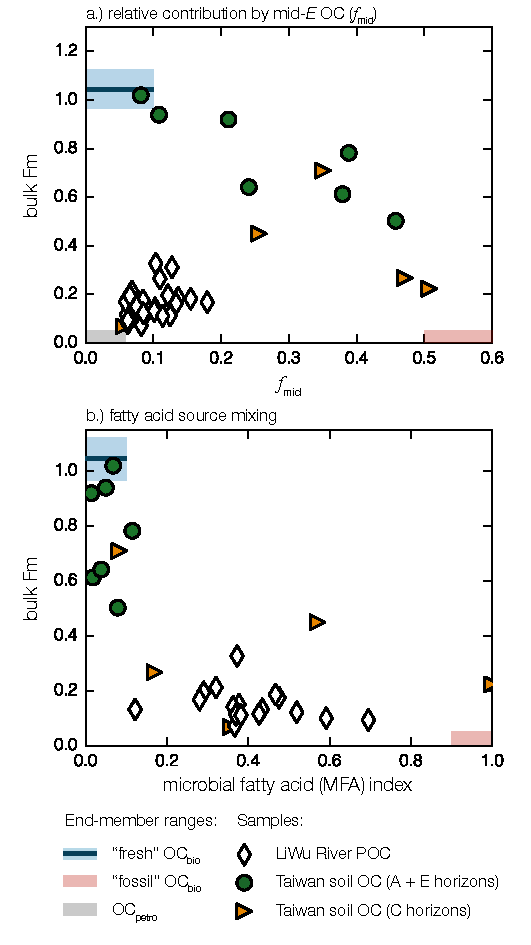
\includegraphics[]{Thesis_Figures/Ch6Fig3}}
	\caption[$f_{\text{mid}}$ and MFA index vs. Fm mixing plots]{\textit{(A)} Relationship between bulk Fm and the relative amount of material contained in the mid-$E$ region ($150 \leq E < 185$ \si{kJ.mol^{-1}}; $f_{\text{mid}}$) for LiWu River POC (white diamonds), C-horizon soil (orange triangles), and A+E-horizon soil (green circles) samples (Table \ref{Ch6Tab:S1}, \ref{Ch6Tab:S2}, \ref{Ch6Tab:S7}). End-member regions are plotted as a blue envelope for fresh OC\sub{bio} (Fm\sub{bio} = \num{1.045 \pm 0.079}; $f_{\text{mid}} \leq 0.1$; Table \ref{Ch6Tab:S5}, \ref{Ch6Tab:S7}), a red box for fossil OC\sub{bio} (Fm $\equiv 0.0$; $f_{\text{mid}} \geq 0.5$), and a gray box for OC\sub{petro} (Fm $\equiv 0.0$; $f_{\text{mid}} \leq 0.04$). \textit{(B)} Relationship between bulk Fm and the microbial fatty acid (MFA) index for all LiWu River POC (white diamonds), C-horizon soil (orange triangles), and A+E-horizon soil (green circles) samples in which alkanoic acids were extracted (Table \ref{Ch6Tab:S1}--\ref{Ch6Tab:S3}). End-member regions are plotted as a blue envelope for fresh OC\sub{bio} (Fm\sub{bio} = \num{1.045 \pm 0.079}; MFA $\leq 0.1$; Table \ref{Ch6Tab:S5}) and a red box for fossil OC\sub{bio} (Fm $\equiv 0.0$; MFA $\geq 0.9$).}
	\label{Ch6Fig:3} 
\end{figure}

The presence of fossil OC\sub{bio} is further supported by alkanoic acid concentrations and \ce{\delta^{13}C} values in both soils and POC. Bulk Fm values correlate negatively with the microbial fatty acid (MFA) index, a proxy for the relative amount of heterotrophic (\textit{i/a}-C\sub{15}) and autotrophic ($\Sigma$LC\sub{24+}) alkanoic acids (Figure \ref{Ch6Fig:3}B; Supplementary Discussion \ref{Ch6SD5}). While we do not expect mixing to be linear in this plot due to production biases \citep{Hemingway:2016bq}, this clearly indicates a high abundance of heterotrophically derived alkanoic acids in samples containing predominantly \ce{^{14}C}-free OC. \ce{\delta^{13}C} values of $\Sigma$LC\sub{24+} \textit{n}-alkanoic acids extracted from A+E-horizon soils correlate strongly with bulk \ce{\delta^{13}C} values (R\super{2} $= 0.959$; $p$-value $< 0.001$, $n = 7$; Table \ref{Ch6Tab:S4}), consistent with the predominance of fresh OC\sub{bio} in these samples. In contrast, the lack of a significant relationship between \textit{i/a}-C\sub{15} and $\Sigma$LC\sub{24+} \ce{\delta^{13}C} values (R\super{2} $= 0.241$; $p$-value $= 0.25$, $n = 7$) indicates that OC\sub{bio} cannot be the sole substrate for heterotrophic organisms \citep{Blair:1985ti}. Rather, this indicates a secondary carbon source to \textit{i/a}-C\sub{15} -- specifically, OC\sub{petro}.

The fact that this mechanism is observed within the saprolites indicates that the kinetic limitation of OC\sub{petro} oxidation is not reached in Taiwanese soils, despite high erosion rates and short residence times within the weathering front \citep{Dadson:2003kl}. OC\sub{petro} oxidation appears to be microbially mediated, supporting laboratory results that suggest \ce{^{14}C}-free material is incorporated into biomass \citep{Petsch:2001eq,Petsch:2005gd} and emphasizing the importance of biology during primary soil succession \citep{Brantley:2011ku}. We therefore expect erosion to exhibit a first-order control on \ce{CO2} emission fluxes due to OC\sub{petro} weathering, as increased erosion will lead to more rapid exposure of bedrock to the weathering front. The \ce{CO2} emission flux calculated here represents a minimum estimate, as fossil OC\sub{bio} is likely less stable than unweathered OC\sub{petro} and could thus be further oxidized.

Erosion additionally governs negative atmospheric \ce{CO2} concentration feedbacks via OC\sub{bio} burial \citep{FranceLanord:1997ua,Galy:2007ev} and weathering of silicate rocks \citep{West:2012cp,Maher:2014kq}. However, the sensitivity of microbial OC\sub{petro} oxidation to changing erosion rates likely differs from that of these \ce{CO2} sinks. The data presented here suggest that OC\sub{petro} weathering flux should increase linearly with erosion rate so long as the catchment-averaged incision depth does not exceed the soil thickness, at which point further increases in erosion will only lead to higher export of unweathered OC\sub{petro} \citep{Hilton:2011jw}. By considering the sensitivity of all of these processes, we propose that erosion rate is the primary control determining the net effect of river catchments as an atmospheric \ce{CO2} source or sink.

\clearpage

\section{Supplementary Material}

\subsection{Methods}\label{Ch6M}

\subsubsection{Sample collection}

LiWu River total suspended sediment (TSS) samples were collected from the surface of the river at the Lushan gauging station (\ang{24.179} N, \ang{121.492} E). The roughness of the channel cross-section (due to large boulders and bedrock canyon walls), combined with steep channels, results in suspended sediments that are well-mixed throughout the water column \citep{Turowski:2008iz}. For each sample, a known volume of water was collected into pre-rinsed HDPE bottles. TSS were isolated by filtering through \SI{0.2}{\micro m} nylon membrane filters, transferred into petri dishes, dried at \SI{60}{\celsius}, and stored in the dark until further analysis. Two samples during the peak of Typhoon Fung Wong contained coarse rock material that was separated and analyzed independently by sieving at \SI{2}{mm}. Before further analysis, \SI{\geq 2}{mm} fractions were rinsed with \SI{3}{\%} hydrogen peroxide at room temperature in a sonic bath to remove any fine-grained material from the surface of each rock, and all rocks from each sample were homogenized together with an agate mortar and pestle. We additionally include a previously described sample from the peak of Typhoon Mindulle collected similarly on 3 July 2004 \citep{Hilton:2008fo,Hilton:2010cg}. Soil samples were obtained as detailed in \citet{Hilton:2013kq}. In summary, \SI{\approx 500}{cm^{3}} of each sample was collected over \SI{10}{cm} intervals, placed into sterile bags, dried at \SI{80}{\celsius}, homogenized, and stored in the dark until analysis.

\subsubsection{Bulk analysis}

TSS were analyzed for organic carbon (\%OC) content and stable isotope composition (\ce{\delta^{13}C}) following the methods of \citet{Whiteside:2011jea} after being ground and homogenized using an agate mortar and pestle. Triplicate aliquots were weighed into silver boats and decarbonated over 12N \ce{HCl} fumes at \SI{60}{\celsius} for 72 hours before measurement using a Fisons elemental analyzer (EA) coupled to a Finnigan Delta\super{plus} isotope ratio mass spectrometer (EA--IRMS). \ce{\delta^{13}C} values are reported in per mille (\si{\permil}) notation relative to Vienna Pee Dee Belemnite (VPDB). Aliquots of TSS for bulk particulate OC (POC) radiocarbon content were decarbonated following the fumigation procedure described above, transferred to pre-combusted (\SI{850}{\celsius}, 5 hours) quartz tubes, evacuated and flame sealed using standard vacuum line techniques, and combusted to \ce{CO2} at \SI{850}{\celsius} for 5 hours. Resulting \ce{CO2} was then quantified manometrically and radiocarbon content was measured at the National Ocean Sciences Accelerator Mass Spectrometry (NOSAMS) facility following standard procedures \citep{McNichol:1994ty,Pearson:1998vy}. Data are reported using fraction modern (Fm) notation following Stuiver and Polach (1977) and corrected for procedural blank contamination. Fm values are not corrected for decay since sample correction [\textit{i.e.} they are identical to the "\ce{^{14}a_{N}}" notation of \citet{Mook:1999vf} and the "\ce{F^{14}C}" notation of \citet{Reimer:2004th}]. To compare bulk and Ramped PyrOx (RPO) isotope results as a check for RPO isotope mass balance, all samples in which RPO isotopes were calculated were re-analyzed for \%OC, \ce{\delta^{13}C}, and Fm after fumigation followed by rinsing with \SI{\approx 5}{mL} \SI{18.2}{M \ohm} MilliQ \ce{H2O} three times to remove residual chlorine \citep{Hemingway:2016rc}. While slight differences exist between \%OC, \ce{\delta^{13}C}, and Fm measured using various acid treatment methods [\textit{i.e.} liquid acid treatment \citep[bulk soils;][]{Hilton:2010cg,Hilton:2013kq}, fumigation (bulk TSS; this study), and fumigation plus rinsing (RPO analysis; this study)], all results between all methods are well correlated (R\super{2} $\geq 0.98$) slopes statistically identical to unity.

\subsubsection{Ramped PyrOx (RPO)}

Decarbonated and rinsed TSS and soil samples were analyzed for RPO thermal lability profiles and corresponding "binned" isotope composition following \citet{Hemingway:2016rc} using \SI{\approx 250}{mg} aliquots and a ramp rate of \SI{5}{\celsius.min^{-1}}. Between each sample, \ce{CO2} concentrations were calibrated using a 2-point calibration curve, while a laboratory working standard was analyzed periodically to check for drift in temperature measurements. All samples were binned into 3 to 7 RPO fractions and \ce{CO2} was re-combusted with \SI{\approx 100}{mg.\ce{CuO}} and \SI{\approx 10}{mg.\ce{Ag}} pellets at \SI{525}{\celsius} for 1 hour to remove residual sulfur-containing gases. \ce{CO2} \ce{^{14}C} content was measured either at NOSAMS or at ETH Zurich using a Mini Carbon Dating System \citep[Micadas;][]{McNichol:1994ty,Christl:2013ks}. Resulting Fm composition was corrected for blank carbon contribution as described in \citet{Hemingway:2016rc}.

\subsubsection{Alkanoic acid extraction and purification}

All soil samples and all TSS samples with \SI{\geq 2.5}{g} of remaining material were extracted for biomarker measurements following the methods described in \citet{Hemingway:2016bq}. Samples were extracted in \SI{20}{mL} of $9:1$ dichloromethane (DCM):methanol (MeOH) in a microwave accelerated reaction system (MARS, CEM corporation) for 20 min at \SI{100}{\celsius}. Lipid extracts were then saponified in \SI{0.5}{mol.L^{-1}} \ce{KOH} in MeOH at \SI{70}{\celsius} for 2 hours to cleave wax esters after the addition of \SI{\approx 1}{\%} \SI{18.2}{M \ohm} MilliQ water in order to prevent methylation of carboxylic acid functional groups. \SI{15}{mL} of MilliQ water was then added, and "base" fractions were liquid--liquid extracted in \SI{5}{mL} of pure hexane 5 times. HCl was then added dropwise until pH 2 was reached and "acid" fractions were liquid--liquid extracted in $4:1$ hexane:DCM until the organic phase was clear. Both fractions were purified over \SI{1}{g} of Supelclean amino-propyl silica gel (Supelco Analytical) using the following elution scheme: \SI{4}{mL} hexane (F1); \SI{7}{mL} $4:1$ hexane:DCM (F2); \SI{10}{mL} $9:1$ DCM:acetone (F3); and \SI{14}{mL} \SI{2}{\%} formic acid in DCM (F4). Acid and base fractions containing alkanoic acids (F4) were then recombined and trans-esterified in \SI{15}{mL} of $95:5$ MeOH:HCl at \SI{70}{\celsius} C for 12 hours. \SI{15}{mL} MilliQ water was then added and fatty acid methyl esters (FAMES) were liquid--liquid extracted into $4:1$ hexane:DCM five times. Finally, FAMES were further purified over \SI{1}{g} amino-propyl silica gel eluted with \SI{4}{mL} hexane (F4\sub{T}F1) and \SI{7}{mL} $4:1$ hexane:DCM (F4\sub{T}F2). After quantification but before isotope measurements, unsaturated FAMES were removed using \SI{0.5}{g} silver nitrate silica gel (Supelco Analytical) in a Pasteur pipette column eluted with: \SI{5}{mL} hexane (SN1) and \SI{18}{mL} $4:1$ hexane:DCM (SN2). Saturated FAMES are thus contained in fraction F4\sub{T}F2, SN2.

\subsubsection{Alkanoic acid quantification and isotope measurement}

FAMES were quantified using a Hewlett Packard 5890 gas chromatograph equipped with a flame ionization detector (GC--FID) and a Gerstel PTV injection system. Chromatographic separation was achieved using a VF-1 capillary column (Agilent Technologies) and the following temperature program: ramp to \SI{130}{\celsius} at \SI{30}{\celsius.min^{-1}}; ramp to \SI{320}{\celsius} at \SI{8}{\celsius.min^{-1}}; hold at \SI{320}{\celsius} for 7.5 min. Samples were analyzed as single injections, quantified using an external standard injected at 3 concentrations between every 5 samples, and normalized to the extracted OC mass. Uncertainty was calculated using the standard deviation of the external sample calibration curve.

Alkanoic acid \ce{\delta^{13}C} was measured using a Agilent 6190 GC coupled with a Finnigan Delta\super{plus} IRMS operated with a combustion interface using \ce{O2} trickle flow. Instrument drift was corrected using pulses of \ce{CO2} with known isotope composition introduced between analyte peaks and \ce{\delta^{13}C} values were further calibrated using an external working standard injected between every \numrange{\approx 5}{10} samples. All samples were injected in triplicate and analytical uncertainty was generally better than \SI{0.3}{\permil}. \ce{\delta^{13}C} values for all homologues were corrected for the isotope composition of trans-esterification methanol. The average of long-chain vascular-plant-derived \textit{n}-alkanoic acids ($\Sigma$LC\sub{24--34}) was calculated as the weighted mean of \textit{n}-C\sub{24} through \textit{n}-C\sub{34} (even homologues only), including propagation of associated uncertainty.

Individual alkanoic acid homologues were separated for radiocarbon analysis using a preparatory column GC (PCGC) as described in \citet{Galy:2011hk}. Between 50 and 100 consecutive injections were made into either a Hewlett Packard 5890 or an Agilent 7890 GC equipped with a RTX- 1 column (Restek Corporation) and a 6-port Gerstel fraction collector (glass traps pre-combusted at \SI{450}{\celsius} for 4 hours). Purified homologues were recovered into \SI{4}{mL} of DCM and further purified over \SI{0.5}{g} silica gel activated with \SI{1}{\%} MilliQ water. Homologue purity was checked by injecting a small amount onto a GC-FID. Similar to bulk measurements, purified homologues were packed into pre-combusted quartz tubes (\SI{850}{\celsius}, 5 hours) with \SI{\approx 150}{mg} copper oxide, evacuated using a vacuum line, and oxidized to \ce{CO2} at \SI{850}{\celsius} for 5 hours. Resulting \ce{CO2} was quantified manometrically and \ce{^{14}C} content was measured at ETH Zurich using a Micadas as described in \citet{Christl:2013ks}. Resulting Fm values were corrected for the known isotope composition of trans-esterification methanol and for blank contamination during the PCGC and combustion procedure as described in \citet{Fornace:2016th}, including uncertainty propagation.

\subsubsection{Data treatment}

Uncertainty on all individual measurements represents propagated analytical error. RPO thermograms are interpreted as a continuum of parallel first-order decay processes, and corresponding activation energy ($E$) distributions were calculated following the inverse method of Chapter \ref{Ch3} using the 'rampedpyrox' Python package \citep{Hemingway:bA3-kvLz}. For plant-wax \textit{n}-alkanoic acids, the average chain length (ACL) was calculated as:
%
% Equation 1
\begin{equation}\label{Ch6Eq:1}
\text{ACL} = \frac{24\times[\ce{C}_{24}] + 26\times[\ce{C}_{26}] + 28\times[\ce{C}_{28}] + 30\times[\ce{C}_{30}] + 32\times[\ce{C}_{32}] + 34\times[\ce{C}_{34}]}{\Sigma \text{LC}_{24-34}}
\end{equation}
%
where $[\text{C}_{j}]$ is the concentration of the $j$-carbon chain-length \textit{n}-alkanoic acid and $\Sigma \text{LC}_{24-34}$ refers to the concentration of even-numbered homologues only. Similarly, the carbon preference index (CPI) was calculated following:
%
% Equation 2
\begin{equation}\label{Ch6Eq:2}
\text{CPI} = \frac{1}{2} \left( \frac{\Sigma \text{LC}_{24-34}}{\Sigma \text{LC}_{23-33}} + \frac{\Sigma \text{LC}_{24-34}}{\Sigma \text{LC}_{25-35}} \right)
\end{equation}
%
where $\Sigma \text{LC}_{23-33}$ and $\Sigma \text{LC}_{25-35}$ refer to even-numbered homologues only. Lastly, the microbial fatty acid (MFA) index was calculated as the ratio of microbial-specific homologues relative to microbial- and plant-wax- specific homologues:
%
% Equation 3
\begin{equation}\label{Ch6Eq:3}
\text{MFA} = \frac{[\text{\textit{i}-C}_{15}] + [\text{\textit{a}-C}_{15}]}{[\text{\textit{i}-C}_{15}] + [\text{\textit{a}-C}_{15}] + \Sigma \text{LC}_{24-34}}
\end{equation}
%
where $[\text{\textit{i}-C}_{15}]$ is the concentration of \textit{iso}-C\sub{15} and $[\text{\textit{a}-C}_{15}]$ is the concentration of \textit{anti iso}-C\sub{15}. All data analysis was performed in the Python programming language version 3.5. and all geospatial analysis was performed in Esri ArcGIS version 10.3.

\subsection{Discussion}

\subsubsection{Site Description}\label{Ch6SD1}

The Central Range was formed by the collision of the Luzon arc on the Philippine Sea Plate with the Eursian continental margin driving uplift rates of \SIrange{5}{7}{mm.yr^{-1}} \citep{Teng:1990tu,Dadson:2003kl}. Taiwan's location in the subtropical western Pacific results in a high frequency of tropical cyclone (typhoon) landfall (\numrange{\approx 2}{3} typhoons per year). This climatic and tectonic setting results in rivers draining the eastern flank of the Central Range that exhibit some of the highest total suspended sediment (TSS) yields in the world, reaching values greater than \SI{10000}{t.km^{-2}.yr^{-1}} \citep{Dadson:2003kl}. Such high sediment transport rates are due to a combination of river incision and bedrock landsliding on steep (threshold) mountain slopes \citep{Hovius:2000ht}, leading to estimated average denudation rates across the eastern Central Range of \SIrange{3}{6}{mm.yr^{-1}} \citep{Dadson:2003kl}. Storm-driven mass wasting events act to efficiently transfer surface vegetation and soils from hillslopes into the river network, leading to high export of biospheric organic carbon \citep[OC\sub{bio};][]{Hilton:2008fo}. Particulate OC\sub{bio} (POC\sub{bio}) export rates in the suspended load have been estimated to be \SI{21 \pm 10}{t.C.km^{-2}.yr^{-1}} \citep{Hilton:2012dt}, amongst the highest in the world \citep{Galy:2015fx}. These rates impose an upper bound on the residence time of surface soil of \SI{\approx 800}{yr} based on the OC\sub{bio} stock in soil and vegetation in Taiwan \citep{Hilton:2012dt}.

High rates of soil erosion and landscape turnover by bedrock landslides \citep{Hovius:2000ht,Lin:2008fy,Hilton:2012dt} results in a continuous exposure of bedrock material to chemical weathering \citep{Hilton:2012dt,Emberson:2016fp}. The dominant lithologies are meta-sedimentary, decreasing in metamorphic grade from the Tananao schist on the east (peak metamorphic temperature \SI{\approx 500}{\celsius}) to the Lushan sedimentary formation on the west \citep[\SI{\leq 150}{\celsius}; Figure \ref{Ch6Fig:S1};][]{Beyssac:2007wg}. As such, bedrock formations contain rock-derived ("petrogenic") organic carbon (OC\sub{petro}), with geological formation average OC\sub{petro} content ranging from \SI{0.19 \pm 0.13}{\%} (Tananao schist; $\mu \pm 2\sigma$) to \SI{0.41 \pm 0.15}{\%} \citep[Lushan formation;][]{Hilton:2010cg}. Bedrock landsliding and incision processes typically mobilize deeper than saprolites and weathered soils \citep{Larsen:2010dr}, meaning that high erosion rates by landslides can supply unweathered OC\sub{petro} to rivers. Indeed, the rate of OC\sub{petro} export in the suspended load of Taiwanese rivers is amongst the highest in the world at \SI{82}{t.C.km^{-2}.yr^{-1}} on average across Taiwan \citep{Hilton:2011jw}. The OC\sub{petro} content of river suspended load suggests that OC\sub{petro} oxidation prior to erosion is \SI{\leq 15}{\%} of this flux (\textit{i.e.} an oxidization rate of \SI{\leq 12}{t.C.km^{-2}.yr^{-1}}). Using the riverine flux of dissolved rhenium as a proxy for OC\sub{petro} oxidation during weathering, \citet{Hilton:2014dh} concluded that catchments in the Central Range oxidize between \SI{7}{tOC\sub{petro}.km^{-2}.yr^{-1}} and \SI{13}{tOC\sub{petro}.km^{-2}.yr^{-1}} to \ce{CO2}. Measured dissolved rhenium yield in these catchments correlated positively with TSS yields, suggesting that OC\sub{petro} weathering rates increase with increasing exposure rate of uplifted bedrock to the surface.

Here, our soil sample set includes both surface horizons containing humified organic material (A+E) as well as the corresponding underlying saprolite (C) horizons containing OC\sub{petro} that has undergone various degrees of oxidation. In addition to soils, we analyze TSS collected from LiWu River, which provide a mixture of weathering and erosion products from throughout the \SI{435}{km.^{2}} catchment. Samples were collected during typhoon Mindulle in 2004 and during three successive typhoon events (Fung Wong, Sinlaku, and Jangmi) between 4 June and 1 October 2008. Draining the Tananao schist, Pilushan, and Lushan sedimentary formations, the LiWu River provides a range of OC\sub{petro} sources that is representative of the Central Range \citep{Hilton:2010cg}.

\subsubsection{Ramped PyrOx data interpretation}\label{Ch6SD2}

In order to relate RPO thermogram results (which inherently depend on experimental conditions such as oven ramp rate) into an intrinsic property of OC chemical bonding environment, we use the inverse distributed activation energy model (DAEM) as described in Chapter \ref{Ch3}. By treating a complex OC mixture as a superposition of parallel first-order decay reactions that are governed by the Arrhenius equation, this model generates a probability density function (pdf) of activation energy [$p_{0}(E)$] that can describe the observed RPO thermogram. Importantly, this does not require any \textit{a priori} assumptions about the distribution of $E$, but rather determines the non-parametric solution to the regularized, non-negative inverse problem \citep[][Chapter \ref{Ch3}]{Forney:2012dr,Forney:2012hz}. However, the inverse DAEM does require that the Arrhenius pre-exponential ("frequency") factor be prescribed \textit{a priori}. Following Chapter \ref{Ch3}, and to properly compare $p_{0}(E)$ between samples, here we choose a constant value of $k_{0}$ = \SI{e10}{s.^{-1}}. Because this inverse method is ill-posed, there exist many possible solutions \citep{Hansen:1994uc}. We choose the best-fit solution that minimizes both $p_{0}(E)$ complexity \citep[as measured by the roughness norm;][]{Forney:2012dr} and residual error using the "L-curve" approach \citep{Tikhonov:1977ui,Hansen:1994uc}. Resulting regularization  values range from $0.01$ to $0.49$. We further calculate the mean $E$ contained within each RPO peak using the evolution of $p_{0}(E)$ throughout each experiment (see Chapter \ref{Ch3} for details).

Because $p_{0}(E)$ is a proxy for chemical composition, mixtures of OC sources with unique molecular structure will result in distinct peaks. For example, POC collected during Typhoon Mindulle is clearly bimodal, with a small peak within the low-$E$ range and a large peak within the high-$E$ range (Figure \ref{Ch6Fig:2}A), consistent with the interpretation that this sample contains a mixture of unweathered OC\sub{petro} and fresh OC\sub{bio} \citep{Hilton:2008fo}. Isotope results for individual RPO fractions further support this interpretation, as low-$E$ OC in this sample is described by an Fm value near $1.0$ while high-$E$ OC is described by Fm near $0.0$ (Table \ref{Ch6Tab:S6}). Mixing of OC end-members with overlapping $E$ distributions will shift points vertically in a plot of isotope composition versus $E$ for each RPO fraction (Figure \ref{Ch6Fig:2}B). That is, source mixing will not shift the end-member $E$ values. Fresh OC\sub{bio} and OC\sub{petro} mixing therefore cannot generate the observed saprolite $p_{0}(E)$ distributions. Rather, this must reflect incorporation of a chemically distinct OC source. We describe this source (fossil OC\sub{bio}) as containing a large amount of OC associated with mid-$E$ values (calculated as the fraction of $p_{0}(E)$ contained between \SIrange{150}{185}{kJ.mol^{-1}}; $f_{\text{mid}}$; Table \ref{Ch6Tab:S7}). Because we have no direct measurement of the $f_{\text{mid}}$ value for this end member, we approximate it using saprolites. Sample TS4 contains no $\Sigma$LC\sub{24+} \textit{n}-alkanoic acids and is described by an Fm value of \num{0.211 \pm 0.002} (Table \ref{Ch6Tab:S2}--\ref{Ch6Tab:S3}), yet still shows clear loss of unweathered OC\sub{petro}. We therefore use the $f_{\text{mid}}$ value of this sample ($0.5$) as the fossil OC\sub{bio} end-member value (Table \ref{Ch6Tab:S7}). Similarly, we use the $f_{\text{mid}}$ value ($0.04$) of \SI{\geq 2}{mm} clasts (sample LW3PETRO) for the OC\sub{petro} end-member and that of high-\%OC surface soils (samples TS5, TS18; $f_{\text{mid}} = 0.11, 0.08$) for the fresh OC\sub{bio} end-member (Table \ref{Ch6Tab:S7}).

Lastly, it has been observed previously that charring can occur within the RPO instrument due to free-radical condensation \citep[Chapter \ref{Ch3}]{Williams:2014bq}. Charring therefore results in an apparent shift toward high $E$ values of otherwise labile OC\sub{bio}. We note that this mechanism is the likeliest cause of high-$E$ fractions in A+E-horizon soils that exhibit Fm values near $0.5$ (Figure \ref{Ch6Fig:2}B). That is, these fractions represent a mixture of thermally stabilized fresh OC\sub{bio} with Fm near $1.0$ and OC\sub{petro} rather than the presence of a biospheric component that has been pre-aged for \SI{\approx 6000}{\ce{^{14}C}.yr}, as the existence of such a component is precluded by the fact that all C\sub{24+} \textit{n}-alkanoic acids contain Fm values $> 0.7$ (mean = \num{1.045 \pm 0.079}; Table \ref{Ch6Tab:S5}). This is further evidenced by the low mass of these fractions, indicating that a small contribution by charred fresh OC\sub{bio} \citep[\SI{\approx 5}{\%} of low-$E$ material;][]{Williams:2014bq} could lead to large changes in Fm (Table \ref{Ch6Tab:S6}).

\subsubsection{Bulk end-member mixing model}\label{Ch6SD3}

To calculate the predicted bulk soil Fm as a function of the difference between soil \%OC and initial bedrock \%OC ($\Delta$\%OC) for a given Fm\sub{bio}, \%OC\sub{petro} initially present in the bedrock (\%OC\sub{br}), and fraction of \%OC\sub{br} that has been oxidized during soil formation ($f_{\text{ox}}$), we use a two end-member mixing model following the equation:
%
% Equation 4
\begin{equation}\label{Ch6Eq:4}
	\text{Fm}\times \text{\%OC} = \text{Fm}_{\text{bio}}\times \text{\%OC}_{\text{bio}} + \text{Fm}_{\text{petro}}\times \text{\%OC}_{\text{petro}}
\end{equation}
%
where Fm\sub{petro} $\equiv 0.0$ by definition. Replacing \%OC\sub{bio} with (\%OC -- \%OC\sub{petro}), \%OC with ($\Delta$\%OC + \%OC\sub{br}), and \%OC\sub{petro} with $(1 - f_{\text{ox}})\times$\%OC\sub{br} and rearranging, this becomes: 
%
% Equation 5
\begin{equation}\label{Ch6Eq:5}
	\text{Fm} = \text{Fm}_{\text{bio}} \left( \frac{\Delta \text{\%OC} + \text{\%OC}_{\text{br}} \times f_{\text{ox}}}{\Delta \text{\%OC} + \text{\%OC}_{\text{br}}} \right)
\end{equation}
%
Because C\sub{24+} \textit{n}-alkanoic acids are known to be produced exclusively by vascular plants \citep[see][for review]{Eglinton:2008hs}, we estimate the average Fm\sub{bio} for our sample set as the precision-weighted mean and standard deviation of C\sub{24+} \textit{n}-alkanoic acid Fm values (Table \ref{Ch6Tab:S5}). By weighting by precision (\textit{i.e.} ignoring concentration), we choose to allow for a maximum range in Fm\sub{bio}, as the samples with the highest Fm content typically contain the highest \textit{n}-alkanoic acid concentrations. However, weighting by precision and concentration results in an identical mean Fm\sub{bio} of \num{1.053 \pm 0.063} (Table \ref{Ch6Tab:S5}). We note that total Fm\sub{bio} might be slightly different than that of C\sub{24+} \textit{n}-alkanoic acids if there exist biases in remineralization rates between between biospheric OC components \citep[\textit{e.g.}][]{Cranwell:1981vg,Meyers:1993vwa}. However, in order to fit bulk Fm values of high-\%OC samples, this model requires that Fm\sub{bio} must be higher than $0.94$ (Table \ref{Ch6Tab:S2}), consistent with our \textit{n}-alkanoic-acid based estimate.

We calculate $\Delta$\%OC for each soil sample using the measured bulk \%OC and corresponding bedrock pair (where available) or formation average value (Table \ref{Ch6Tab:S2}). We then calculate the best-fit value of $f_{\text{ox}}$ by minimizing the root mean square error (RMSE) between the model fit and measured values using an average \%OC\sub{br} value for the entire dataset [\SI{0.36 \pm 0.16}{\%}]. Uncertainty is propagated by again calculating the best-fit $f_{\text{ox}}$ value using Fm\sub{bio} $= \mu + \sigma$ and Fm\sub{bio} = $= \mu - \sigma$, where $\mu$ and $\sigma$ are the mean and standard deviation of precision-weighted Fm\sub{bio}. Because we explicitly include \%OC\sub{br} uncertainty when estimating OC\sub{petro} oxidation fluxes (Supplementary Discussion \ref{Ch6SD4}), this is omitted here.

\subsubsection{Flux estimate}\label{Ch6SD4}

The results presented here indicate that OC\sub{petro} oxidation can keep pace with the high rates of physical denudation and mineral supply that occur in tectonically active mountain belts such as Taiwan \citep{Dadson:2003kl}. To compare this process to acid-hydrolysis driven silicate weathering rates and other geological carbon fluxes, we seek to estimate OC\sub{petro} oxidation rate occurring in soils. The soils from the Central Range Taiwan show that, on average, $73^{+2}_{-3}$ \% of initial OC\sub{petro} present in the bedrock is lost during soil formation (Figure \ref{Ch6Fig:1}; Supplemental Discussion \ref{Ch6SD2}). This depletion can be used to estimate the OC\sub{petro} oxidation flux according to:
%
% Equation 6
\begin{equation}\label{Ch6Eq:6}
	\Phi_{\text{petro}} = \frac{\mean{[\text{OC}_{\text{petro}}]} f_{\text{ox}} \rho_{\text{soil}} z_{\text{soil}}}{\tau}
\end{equation}
%
where $\Phi_{\text{petro}}$ is the flux of \ce{CO2} to the atmosphere due to OC\sub{petro} oxidation in soils (\si{t.C.km^{-2}.yr^{-1}}), $\mean{[\text{OC}_{\text{petro}}]}$ is the average amount of OC\sub{petro} initially present in the bedrock (Table \ref{Ch6Tab:S2}), $f_{\text{ox}}$ is the fraction of OC\sub{petro} that is oxidized in soils (Figure \ref{Ch6Fig:1}), $\rho_{\text{soil}}$ is the soil density (\si{t.km^{-3}}), $z_{\text{soil}}$ is the depth of the weathering zone (\si{m}), and $\tau$ is a measure of the residence time within the weathering zone.

We use the measured saprolite soil samples to constrain $z_{\text{soil}}$, as these indicate that OC\sub{petro} loss occurs at depths of \SIrange{0.2}{0.9}{m} (Table \ref{Ch6Tab:S2}), consistent with measurements of average saprolite thickness from Taiwan \citep{Tsai:2001vp}. In the absence of direct measurements of soil formation rate \citep[\textit{e.g.}][]{Larsen:2014gq}, we estimate  using three independent approaches in order to constrain a range of possible values:

\begin{enumerate}[label=(\textit{\roman*})]
%
\item First, we calculates  by acknowledging landslides as the dominant geomorphic agent with respect to erosion of the landscape. Assuming landslide depth is deeper than that of the weathering front \citep[\SI{\approx 0.8}{m};][]{Tsai:2001vp}, landsliding imposes a timescale over which the surface area of a mountain catchment is refreshed (\textit{i.e.} the average time between landslides at a given location). We compile measured rates of landsliding in Taiwan (RL, in \% of catchment area per year) for four catchments where data are available \citep[Table \ref{Ch6Tab:S8};][]{Chang:2002wr,Chang:2007fm,Lin:2008fy,Chen:2013eh,Chen:2015hs}. There can be considerable variability at the annual-timescale in landslide rates \citep{Lin:2008fy} due to extreme landslide triggers, such as the 1999 Chi-Chi Earthquake \citep{Hovius:2011kc} and the 2009 Typhoon Morakot \citep{West:2011eo}. These events are likely to have return intervals of several decades to centuries. Therefore, to capture a more representative value of landslide-driven catchment turnover, we use data on landslide rate outside these extreme events, giving annual average values of \SIrange{0.14}{1.62}{\%.yr^{-1}}, thus corresponding to a $\tau$ value of \SIrange{62}{711}{yr}.
%
\item Next, we use the catchment-wide denudation rates ($\epsilon$; \si{mm.yr^{-1}}) as measured in the solid and dissolved loads of rivers, which in Taiwan varies from \SIrange{\approx 3}{6}{mm.yr^{-1}} \citep{Dadson:2003kl}. This provides a minimum estimate of $\tau$ (and hence an upper estimate of OC\sub{petro} oxidation flux) since it does not acknowledge the fact that much of the physical denudation occurs by bedrock landslides \citep{Hovius:2000ht}, which erode deeper than the typical saprolite thickness in Taiwan \citep[\textit{i.e.} \SI{\approx 0.8}{m};][]{Tsai:2001vp,Larsen:2010dr}. This process results in the export of unweathered OC\sub{petro} that did not reside in the surface weathering zone prior to erosion and transport. We then calculate $\tau = \frac{z_{\text{soil}}}{\epsilon}$, with results ranging from \SIrange{50}{266}{yr}.
%
\item Finally, we consider the surface erosion rates as constrained by the inventory of OC\sub{bio} on hillslopes (total stock \SIrange{5000}{9000}{t.C.km^{-2}}) divided by OC\sub{bio} discharge flux in rivers \citep[\SIrange{11}{31}{t.C.km^{-2}.yr^{-1}};][]{Hilton:2012dt}. This method places an upper bound on the residence time of organic matter in Taiwanese soils (and hence a lower estimate of OC\sub{petro} oxidation) for two reasons: 1) the measured biospheric OC discharge rates are thought to be conservative based on the flux-weighted average method used to quantify them \citep{Hilton:2012dt}, and 2) this inherently ignores any other output processes that would lead to an additional output flux from soils (\textit{i.e.} the denominator must be a minimum).
%
\end{enumerate}

Because most variables inputted into Equation \ref{Ch6Eq:6} are poorly constrained with unknown probability density functions due to a low number of observations, we use a Monte Carlo approach to estimate $\Phi_{\text{petro}}$. We use the area-weighted \%OC\sub{petro} of geological formations contained within the LiWu and WuLu basins to calculate $\mean{[\text{OC}_{\text{petro}}]}$ 
[\SI{0.24 \pm 0.06}{\%}; \citealp{Hilton:2010cg}], while we allow $\rho_{\text{soil}}$ and $z_{\text{soil}}$ to span the known range of possible values [\SIrange{2.0}{2.5}{t.km^{-2}.yr^{-1}} and \SIrange{0.2}{0.9}{m}, respectively; \citealp{Tsai:2001vp}]. As the most conservative estimate, we assign a uniform distribution between the known bounds for all variables and estimate the range of resulting  $\Phi_{\text{petro}}$ values using \num{10000} iterations.

The three independent constraints on  provide estimates of OC\sub{petro} oxidation rate at the catchment scale ranging from \SIrange{5.6}{17.1}{t.C.km^{-2}.yr^{-1}} (median values; Figure \ref{Ch6Fig:S1}A). While these remain uncertain, they are remarkably consistent and provide an order of magnitude quantification of OC\sub{petro} oxidation rate that is similar to two independent previous measurements \citep[Figure \ref{Ch6Fig:S2}B;][]{Hilton:2011jw,Hilton:2014dh}. First, the OC\sub{petro} content of suspended sediments suggest that \SI{\leq 15}{\%} of the OC\sub{petro} exported from the catchment has undergone oxidation \citep{Hilton:2011jw}. For the annual average OC\sub{petro} export of \SI{82}{t.C.km^{-2}.yr^{-1}} in river suspended load from Taiwan \citep{Hilton:2011jw} this suggests an OC\sub{petro} oxidation flux \SI{\leq 12}{t.C.km^{-2}.yr^{-1}}. Second, the trace element rhenium provides a proxy for OC\sub{petro} oxidation \citep{Jaffe:2002wya,Dalai:2002wg} due to its association with organic matter in rocks \citep{Selby:2003iq} and its solubility upon chemical weathering \citep{Colodner:1993tl}. Dissolved Re flux provides an estimate of OC\sub{petro} oxidation rate in Taiwan of \SIrange{7}{13}{t.C.km^{-2}.yr^{-1}}. Together these approaches demonstrate that microbial-induced processing of OC\sub{petro} in soils can sustain high rate of loss and \ce{CO2} release at the catchment scale.

\subsubsection{Alkanoic acid sources and mixing}\label{Ch6SD5}

Carbon preference index (CPI) values for all soil samples containing long-chain \textit{n}-alkanoic acids (C\sub{24+}) range from \numrange{2.73}{5.23} (Table \ref{Ch6Tab:S3}), consistent with a fresh vascular plant source \citep{Eglinton:1967uz}. While concentrations in TSS samples were too low to calculate CPI values, the range of C\sub{24+} average chain lengths (ACL) is statistically identical to that for soils (TSS: \num{26.04 \pm 1.05}; soils: \num{27.41 \pm 1.41}). Because environmental conditions such as temperature and elevation have been shown to affect ACL \citep{Bush:2013ie}, this suggests that our soil sample set captures the entire range of environmental variability that is observed in the catchment-integrated TSS.

Alkanoic acid \ce{\delta^{13}C} values are commonly used to trace the source of OC components such as vascular plants (C\sub{24+} \textit{n}-alkanoic acids) or microbial biomass (\textit{i/a}-C\sub{15}). Here, we compare \ce{\delta^{13}C} between alkanoic acids and bulk OC to understand the source of carbon being incorporated into microbial biomass. Because it has been shown that heterotrophic lipids reflect a consistent, small (\SI{< 3}{\permil}) \ce{^{13}C} fractionation relative to substrate material \citep{Blair:1985ti}, the \ce{\delta^{13}C} of \textit{i/a}-C\sub{15} can be used to distinguish microbial source carbon assuming end-members contain unique \ce{\delta^{13}C} values. However, because both vegetation and bedrock \ce{\delta^{13}C} values span a range of \SI{\approx 10}{\permil} in the Central Range \citep{Hilton:2010cg,Hilton:2013kq}, they cannot be separated based on absolute value. Still, if vascular-plant-derived OC were the sole source of substrate for heterotrophs, then \textit{i/a}-C\sub{15} \ce{\delta^{13}C} values should track those of $\Sigma$LC\sub{24+} \textit{n}-alkanoic acids. This is clearly not observed, as there exists no significant correlation between these compounds in A+E horizon soils (R\super{2} = $0.241$; $p$-value = $0.25$, $n = 7$). Rather, this suggests that microbial biomass, as measured using \textit{i/a}-C\sub{15} alkanoic acids, is sourced from a mixture of bedrock-derived OC\sub{petro} as well as plant-derived fresh OC\sub{bio}.

\clearpage

\subsection{Supplementary Tables}

% Reset table counter
\renewcommand\thetable{\thechapter.S\arabic{table}}    
\setcounter{table}{0}  

% Change caption justification
\captionsetup[table]{justification=raggedright,singlelinecheck=off}

All supplementary tables for this chapter are available on my personal GitHub website at the following link: \url{https://github.com/FluvialSeds/thesis_master}

% Table S1
\begin{table}[h!]
	\caption[Bulk LiWu River POC measurements]{Environmental parameters and bulk data from the LiWu River suspended sediments (\%OC, \ce{\delta^{13}C}, Fm).}
	\label{Ch6Tab:S1} 
\end{table}
%
% Table S2
\begin{table}[h!]
	\caption[Bulk Taiwan soil and bedrock OC measurements]{Environmental parameters and bulk data from Taiwanese soil samples (\%OC, \ce{\delta^{13}C}, Fm).}
	\label{Ch6Tab:S2} 
\end{table}
%
% Table S3
\begin{table}[h!]
	\caption[Alkanoic acid concentrations, ACL, CPI, and MFA]{Alkanoic acid concentrations and metrics ($\Sigma$LC\sub{24--34}, ACL, CPI, MFA) for all available suspended sediments and soils.}
	\label{Ch6Tab:S3} 
\end{table}
%
% Table S4
\begin{table}[h!]
	\caption[Alkanoic acid \ce{\delta^{13}C} values]{Alkanoic acid \ce{\delta^{13}C} values for select suspended sediments and all soils.}
	\label{Ch6Tab:S4} 
\end{table}
%
% Table S5
\begin{table}[h!]
	\caption[\textit{n}-Alkanoic acid Fm values]{\textit{n}-Alkanoic acid Fm values for all soils.}
	\label{Ch6Tab:S5} 
\end{table}
%
% Table S6
\begin{table}[h!]
	\caption[RPO fraction masses, Fm, and $E$ values]{RPO fraction masses, Fm, and $E$ values for select suspended sediments and all soils.}
	\label{Ch6Tab:S6} 
\end{table}
%
% Table S7
\begin{table}[h!]
	\caption[RPO $f_{\text{low}}$, $f_{\text{mid}}$, and $f_{\text{high}}$ metrics for all samples]{RPO $f_{\text{low}}$, $f_{\text{mid}}$, and $f_{\text{high}}$ metrics for all samples.}
	\label{Ch6Tab:S7} 
\end{table}
%
% Table S8
\begin{table}[h!]
	\caption[Literature compilation of landslide rates in Taiwan]{Compilation of all published landslide rates in Taiwan.}
	\label{Ch6Tab:S8} 
\end{table}

% Reset for future chapters
\renewcommand\thetable{\thechapter.\arabic{table}}

% Reset caption justification
\captionsetup[table]{justification=justified}

\clearpage

\subsection{Supplementary Figures}
% Reset figure counter
\renewcommand\thefigure{\thechapter.S\arabic{figure}}    
\setcounter{figure}{0}  

% Supplementary figures

\begin{figure}[h!]
	\makebox[\textwidth][c]{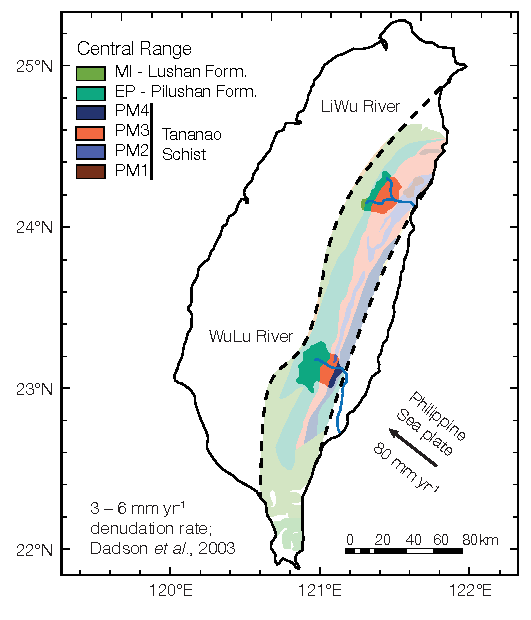
\includegraphics[]{Thesis_Figures/Ch6FigS1}}
	\caption[Lithological map of Taiwan]{Map of Taiwan highlighting the lithology of the Central Range \citep{Chen:2000mp}: Lushan formation (MI; green), Pilushan formation (EP; teal), and Tananao schist (blue, orange, purple, and red). Direction of Philippine Sea Plate tectonic motion is shown as a black arrow \citep{Teng:1990tu}}
	\label{Ch6Fig:S1} 
\end{figure}

\begin{figure}[p]
	\makebox[\textwidth][c]{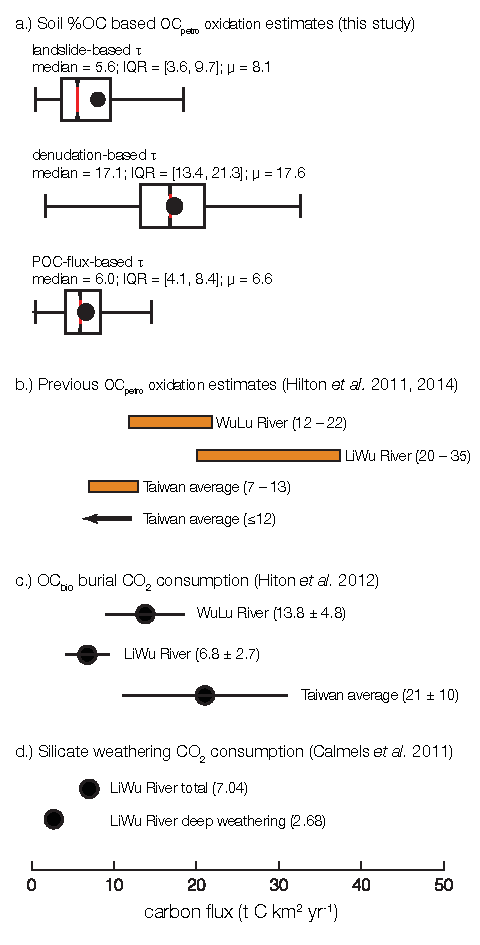
\includegraphics[]{Thesis_Figures/Ch6FigS2}}
	\caption[\ce{CO2} source and sink flux estimates from various processes in the Central Range]{\textit{(A)} Calculated \ce{CO2} emission flux due to OC\sub{petro} oxidation in soils within the LiWu and WuLu catchments using three independent estimates of soil residence time ($\tau$; see Supplementary Discussion \ref{Ch6SD4} for details) represented as box plots (IQR = interquartile range = 25\super{th} to 75\super{th} percentile). \textit{(B)} Previously published estimates using dissolved rhenium as a proxy for oxidized OC\sub{petro} \citep[orange bars;][]{Hilton:2014dh} and based on OC\sub{petro} export yield \citep[black arrow;][]{Hilton:2011jw}. \textit{(C)} Estimates of \ce{CO2} consumption due to OC\sub{bio} export and burial \citep[mean $\pm 1$ std. dev.;][]{Hilton:2012dt}. \textit{(D)} Estimates of \ce{CO2} consumption due to silicate weathering in the LiWu River catchment \citep{Calmels:2011gv}, separated into total flux and flux due to deep chemical weathering only.}
	\label{Ch6Fig:S2} 
\end{figure}

\begin{figure}[p]
	\makebox[\textwidth][c]{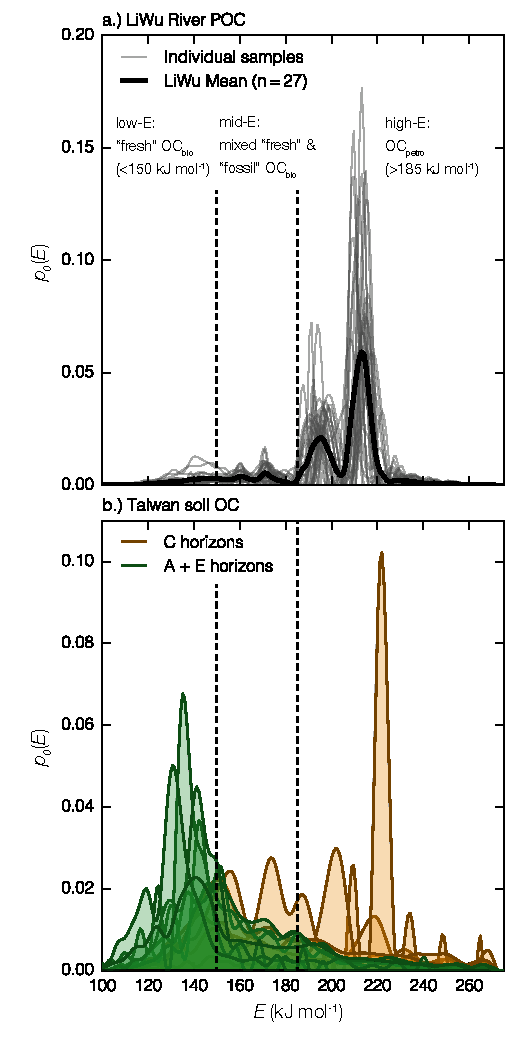
\includegraphics[]{Thesis_Figures/Ch6FigS3}}
	\caption[RPO $p_{0}(E)$ distributions for all samples analyzed]{\textit{(A)} RPO-derived $E$ distributions [$p_{0}(E)$] for all LiWu River POC samples, including \SI{\geq 2}{mm} clasts analyzed separately as a proxy for bedrock OC\sub{petro} ($n = 27$). Individual runs are plotted as thin gray lines, and the mean $p_{0}(E)$ is plotted as a thick black line. \textit{(B)} $p_{0}(E)$ for all C-horizon (orange) and A+E-horizon (green) soil samples analyzed in this study. For both panels, dotted lines separate $p_{0}(E)$ into low-$E$ (\SI{< 150}{kJ.mol^{-1}}), mid-$E$ ($150 \leq E < 185$ \si{kJ.mol^{-1}}), and high-$E$ (\SI{\geq 185}{kJ.mol^{-1}}) regions.}
	\label{Ch6Fig:S3} 
\end{figure}

% Reset figure style for subsequent chapters
\renewcommand\thefigure{\thechapter.\arabic{figure}}
